\chapter{Implementation}
\label{sec:implementation}

\section{Lösungsansatz}
\label{sec:Lösung}

Übergeordnet lässt sich die Aufgabe dieser Arbeit damit zusammenfassen, aus einem Bild Wissen zu ziehen, welches einen hohen Grad an Abstraktion beinhaltet. Da herkömmliche Neuronale Netzwerke alleine nicht für diese Aufgabe ausreichen, wird in dieser Arbeit der Ansatz untersucht, durch die Kombination aus Neuronalem Nerz und semantischem Netzwerk ein System zu schaffen und zu bewerten, welches aus einem Bild Informationen über z.B. die Räumlichkeit und Handlungsfelder, theoretisch aber über jegliches Thema, abstrahieren kann. 


\begin{figure}[h]
	
	\begin{center}
		
		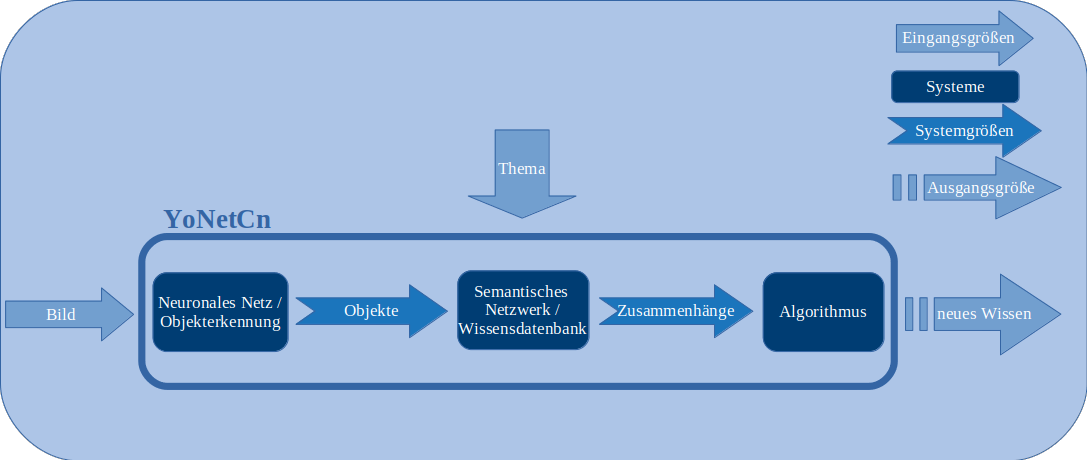
\includegraphics[width=14cm]{images/Masteridee.png}
		
		\caption{Aufbau System YoNetCn}
		
		\label{system_Bild}
		
	\end{center}
	
	
\end{figure}


In Abbildung X.x ist das Konzept für dieses System, welches unter dem Namen YoNetCn zusammengefasst wird, dargestellt. Die primäre Eingangsgröße für YoNetCn ist ein Bild,in welchem durch ein Neuronales Netz Objekte erkannt werden. Die Objekte dienen zusammen mit der sekundären Eingangsgröße, einem Thema oder Themengebiet, einem Semantischen Netz als Eingangsgrößen. Ausgegeben werden vom semantischem Netz als Systemgröße die Zusammenhänge zwischen den Objekten und dem Thema. Ein Algorithmus bewertet und filtert diese Zusammenhänge und schließt daraus auf neues Wissen. Als Beispiel hierfür dient die Szenenerkennung. 



\begin{figure}[h]
	
	\begin{center}
		
		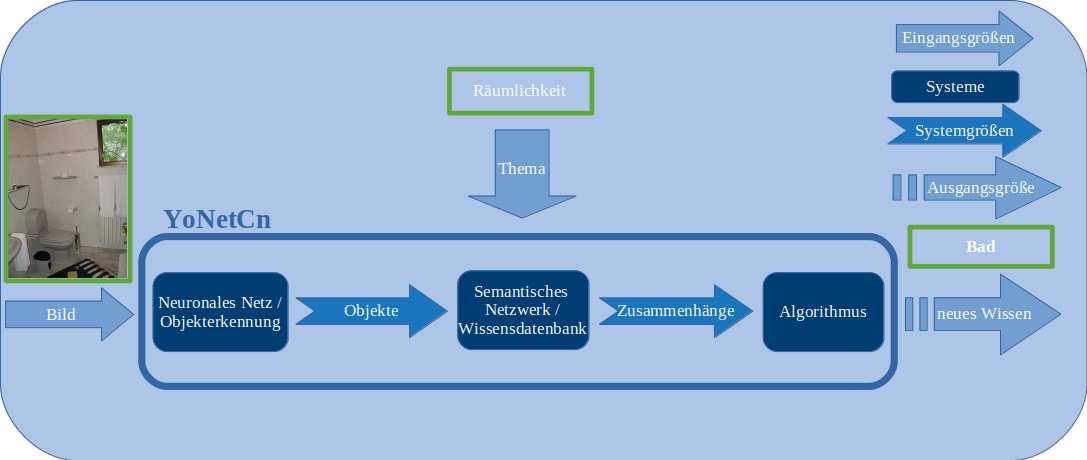
\includegraphics[width=14cm]{images/Masteridee_2.png}
		
		\caption{Szenenerkennung mit YoNetCn}
		
		\label{system_Bild}
		
	\end{center}
	
	
\end{figure}


Abbildung X.x zeigt die Szenenerkennung mit YoNetCn am Beispiel eines Bildes von einem Bad. Wird zu diesem Bild das Thema Räumlichkeit als sekundäre Eingangsgröße eingegeben, so wird als Ausgabe "Bad" ausgegeben. Bei gleichem Bild, jedoch mit sekundärer Eingabe "Tätigkeit", soll YoNetCn Adjektive wie duschen, auf Toilette gehen, oder Zähne putzen ausgeben. Theoretisch sind jegliche sekundären Eingangsgrößen möglich, jedoch wurde sich in dieser Arbeit auf die Themen Räumlichkeit und Tätigkeit beschränkt, da der zeitliche Rahmen dieser Arbeit ansonsten gesprengt werden würde und diese beiden Themengebiete als Nachweis für die grundsätzliche Durchführbarkeit der Aufgabenstellung ausreichen. 


Auf Grundlage des konkreten Anwendungsbereiches von YoNetCn, der Servicerobotik, wurde als Stellgröße die Verarbeitungszeit und die Genauigkeit definiert. Ein Serviceroboter soll in Echtzeit erkennen können, welche Objekte sich in dem  Raum befinden, in welchem Raum er sich befindet und welche Handlungen mit den erkannten Objekten durchführbar sind. Da Echtzeit je nach Anwendungsbereich unterschiedlich ausgelegt wird, müssten für diesen Anwendungsfall genauere Untersuchungen für eine angemessene Reaktionszeit des Roboters durchgeführt werden, was jedoch nicht Umfang dieser Arbeit ist. Für YoNetCn wurde ein Wert von kleiner 10 Sekunden für die Reaktionszeit definiert, der Einfluss der Auslegung von YoNetCn auf die Reaktionszeit wird im Verlauf der Arbeit genauer beschrieben. 

Die Genauigkeit von YoNetCn wird am Beispiel der Räumlichkeit genauer untersucht und es werden verschiedene Stell- und Störgrößen, deren Einfluss auf die Genauigkeit herausgearbeitet.
Als Beispiel hat ein großes Neuronales Netz, welches sehr viele Objekte erkennt, einen positiven Einfluss auf die Genauigkeit, jedoch wird dadurch die Verarbeitungszeit negativ beeinflusst, da größere Netze mehr Rechenoperationen als kleine benötigen. Entsprechend gilt es eine Balance zwischen den beiden Stellgrößen zu finden. 
Semantische Netzwerke basieren auf Sprache. Da Sprache mehrdeutig sein kann und unter Umständen zu Missverständnissen führt, allgemein nicht immer klar definiert ist im Vergleich zur Informatik und Mathematik, wird auch das Zusammenspiel zwischen dem Neuronalen Netz und dem Semantischen Netz untersucht und entsprechende Störgrößen herausgearbeitet. 


